\usetikzlibrary{calc}


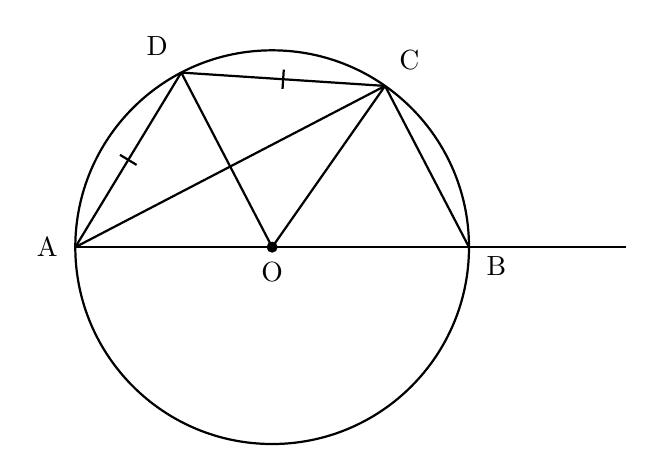
\begin{tikzpicture}[scale=1]

    % Define the center of the circle
    \coordinate (O) at (0,0);
    
    % Define the points on the circle based on the given geometry
    % A is at the leftmost point of the horizontal diameter
    \coordinate (A) at (180:2.5);
    % B is at the rightmost point of the horizontal diameter
    \coordinate (B) at (0:2.5);
    % C is shifted more to the left (set to 55 degrees to match visual preference)
    \coordinate (C) at (55:2.5);
    % D is adjusted to maintain AD = DC (arc AC is 180-55=125 degrees. 125/2 = 62.5. 55+62.5 = 117.5 degrees)
    \coordinate (D) at (117.5:2.5);

    % Draw the circle
    \draw[thick] (O) circle (2.5);

    % Draw the horizontal line extending from A, through O and B, outwards to the right
    \draw[thick] (A) -- (4.5,0);

    % Draw the lines and chords as shown in the image
    \draw[thick] (A) -- (D); % Chord AD
    \draw[thick] (D) -- (C); % Chord DC
    \draw[thick] (C) -- (B); % Chord CB
    \draw[thick] (A) -- (C); % Diagonal AC
    
    % Draw the radius lines to D and C
    \draw[thick] (O) -- (D);
    \draw[thick] (O) -- (C);

    % Draw a prominent dot for the center O
    \fill (O) circle (2pt);

    % Add equal-length tick marks on segments AD and DC
    % Tick mark on the midpoint of AD
    \draw[thick] ($ (A)!.5!(D) ! 3.5pt ! 90:(D) $) -- ($ (A)!.5!(D) ! 3.5pt ! -90:(D) $);
    % Tick mark on the midpoint of DC
    \draw[thick] ($ (D)!.5!(C) ! 3.5pt ! 90:(C) $) -- ($ (D)!.5!(C) ! 3.5pt ! -90:(C) $);

    % Place the labels for all the vertices
    \node[left] at (180:2.6) {A};
    \node[above left] at (117.5:2.6) {D};
    \node[above right] at (55:2.6) {C};
    \node[below right] at (0:2.6) {B};
    \node[below, yshift=-2pt] at (O) {O};

\end{tikzpicture}